\documentclass[a5paper]{article}
\usepackage[a5paper, top=8mm, bottom=8mm, left=8mm, right=8mm]{geometry}

\usepackage{polyglossia}
\setdefaultlanguage[babelshorthands=true]{russian}

\usepackage{fontspec}
\setmainfont{FreeSerif}
\newfontfamily{\russianfonttt}[Scale=0.7]{DejaVuSansMono}

\usepackage[font=scriptsize]{caption}

\usepackage{amsmath}
\usepackage{amssymb,amsfonts,textcomp}
\usepackage{color}
\usepackage{array}
\usepackage{hhline}
\usepackage{cite}
\usepackage{verse}
\usepackage{xcolor}

\usepackage[hang,multiple]{footmisc}
\renewcommand{\footnotelayout}{\raggedright}

\PassOptionsToPackage{hyphens}{url}\usepackage[xetex,linktocpage=true,plainpages=false,pdfpagelabels=false]{hyperref}
\hypersetup{colorlinks=true, linkcolor=blue, citecolor=blue, filecolor=blue, urlcolor=blue, pdftitle=1, pdfauthor=, pdfsubject=, pdfkeywords=}

\usepackage{tabu}

\usepackage{graphicx}
\usepackage{indentfirst}
\usepackage{multirow}
\usepackage{subfig}
\usepackage{footnote}
\usepackage{minted}

\newcommand{\attribution}[1] {
    \vspace{-5mm}\begin{flushright}\begin{scriptsize}\textcolor{gray}{\textcopyright\, #1}\end{scriptsize}\end{flushright}
}

\sloppy
\pagestyle{plain}

\title{Проектирование распределённых приложений, технические вопросы}
\author{Юрий Литвинов\\\small{y.litvinov@spbu.ru}}
\date{01.12.2022}

\begin{document}

\maketitle
\thispagestyle{empty}

\section{Введение}

Подавляющее большинство современных приложений в той или иной степени распределённые. Начиная от простых веб-сайтов, где распределённость сводится к наличию клиента, работающего в браузере или на мобильном телефоне, и простой серверной части, заканчивая огромными распределёнными системами из сотен микросервисов, распределёнными базами данных и системами распределённых высокопроизводительных вычислений типа Apache Spark. При этом при проектировании распределённых приложений следует учитывать массу факторов, связанных с их распределённой структурой: независимые отказы, проблемы согласованности данных, горизонтального масштабирования и т.д. Поэтому проектированию распределённых приложений в этом курсе уделяется особое внимание.

Итак, распределённая система --- это приложение, компоненты которого находятся в компьютерной сети и взаимодействуют друг с другом через обмен сообщениями. Как правило, все компоненты так или иначе работают с какими-то общими ресурсами, которые так же хранятся где-то в сети. Собственно, распределённость и нужна обычно для того, чтобы предоставлять доступ к общим ресурсам сразу нескольким пользователям либо одному пользователю, но с разных устройств, либо организовать эффективную распределённую обработку и хранение информации. При этом есть принципиальные отличия распределённых систем от <<обычных>> приложений (хотя сейчас стоило бы распределённые системы называть обычными).

\begin{itemize}
    \item Распределённые системы принципиально параллельны, и по-другому никак не сделать. Причём, это не <<обычная>> многопоточная параллельность, а многопроцессная, когда компоненты системы не имеют доступа к общей памяти\footnote{В подавляющем большинстве случаев. Есть системы с распределённой памятью, но они очень редки.}, при этом ещё расходы на коммуникацию между процессами весьма значительны.
    \item Каждый компонент распределённой системы --- это отдельный процесс, который может работать или не работать по тем или иным причинам независимо от остальных компонентов (так называемые <<независимые отказы>>). Плюс к тому сеть принципиально ненадёжна, поэтому присутствуют ещё временные отказы, связанные со сбоями работы сети.
    \item Опять-таки по самой природе сети невозможно установить единую для системы последовательность событий (то есть в системе нет единого времени), что может быть критично для поддержания целостности данных. Пакеты могут приходить в разном порядке, в разное время разным адресатам, или не приходить вообще, причём это не ошибка, а вполне нормальная ситуация. Так что два разных компонента могут видеть действия пользователей в совершенно разном порядке, что приводит к проблемам гонок гораздо большего масштаба, чем это обычно случается в многопоточном программировании, и требует гораздо больших усилий, если с этим надо бороться.
\end{itemize}

Вообще, есть даже известный список заблуждений, которые имеют разработчики <<десктопных>> систем, только-только погружающиеся в программирование распределённых систем\footnote{Страница в Википедии: \url{ https://en.wikipedia.org/wiki/Fallacies_of_distributed_computing} (дата обращения: 13.10.2021).}:

\begin{itemize}
    \item сеть надёжна --- нет, она даже при обычном функционировании может терять соединение относительно надолго, поэтому любое сетевое приложение должно уметь восстанавливаться после сетевых ошибок и быть готовым к потере связи с любым из компонентов;
    \item задержка при передаче нулевая, поэтому можно взять монолитное приложение, распилить его на веб-сервисы и в цикле от одного до миллиона слать к веб-сервису запросы;
    \item пропускная способность бесконечна, поэтому идея гонять между сервисами туда-сюда гигабайтные файлы не совсем безумна;
    \item сеть защищена и уж ваш-то сервис никто не будет пытаться взломать --- на самом деле не надо даже злого умысла, нанести ущерб может давно забытый червь, всё ещё влачащий жалкое существование где-то в локалке;
    \item топология сети не меняется, так что если хорошо работало вчера, то будет работать и завтра -- но тут уборщица случайно выдёргивает сетевой кабель из маршрутизатора;
    \item администрирование сети централизовано, поэтому если такой-то порт открыт в локальной сети вашей компании, то открыт и у всех остальных --- однако автор как-то разрабатывал ПО для школ, там обычный пользователь не имеет прав даже на запись на диск;
    \item расходы на передачу данных равны нулю, поэтому можно не закладывать в смету проекта расходы на сетевое оборудование, плату за трафик и аренду инфраструктуры;
    \item сеть однородна, так что можно рассчитывать на одинаковую повсюду среду передачи с одинаковыми физическими свойствами каналов связи --- ни у кого из ваших пользователей нет мобильного или спутникового интернета, например.
\end{itemize}

\section{Архитектура распределённых систем}

Из введения могло сложиться впечатление, что разработка распределённых систем --- чрезвычайно сложная задача. Однако уже успел сложиться набор практик, типовых архитектур и технологий, который при аккуратном использовании позволяет решить многие из проблем и сделать сетевую разработку доступной даже школьникам. Начнём рассмотрение мы с самого низкого уровня, с технологий коммуникации в сетевых приложениях, а в следующей лекции рассмотрим более <<архитектурные>> вопросы.

Для начала рассмотрим, как вообще можно организовать взаимодействие компонентов в распределённой системе. Каждый компонент является независимым приложением, работает как отдельный процесс, но должен активно общаться с остальными компонентами системы. Возможны следующие варианты того, как это устроить.

\begin{itemize}
    \item Межпроцессное взаимодействие средствами ОС, если компоненты расположены физически на одном устройстве. Например, взаимодействие через пайпы или именованные пайпы (в Linux такая схема работы очень популярна, но Windows так тоже умеет), через общие файлы (как правило, плохая идея, потому что есть пайпы --- те же файлы, но без долгой записи на диск). Так может быть организована связь с СУБД, если бизнес-логика и СУБД находятся на одной машине, и это может быть в разы эффективнее, чем сетевое соединение. На самом деле, это не очень распределённый сценарий работы, так что дальше мы его рассматривать не будем.
    \item Механизмы удалённого вызова по сети: простые протоколы <<запрос-ответ>> (например, так работают REST-сервисы, про которые попозже), удалённые вызовы процедур (RPC, Remote Procedure Calls), удалённые вызовы методов (RMI, Remote Method Invocation --- так работают веб-сервисы). Такие механизмы предполагают наличие сетевого соединения (хотя оно вполне может быть с сервером на той же машине --- для универсальности кода и гибкости деплоя, хотя и медленнее и хуже, чем более специализированные для такого случая способы). Кроме того, чаще всего большая часть работы по организации коммуникаций может быть реализована один раз в некоем middleware (например, RPC реализуют известные инструменты gRPC, Apache Thrift, ZeroC ICE), причём такие инструменты поддерживают кодогенерацию клиентской и серверной стороны коммуникаций, так, чтобы прикладной программист мог пользоваться удалёнными методами так же, как и локальными.
    \item Механизмы неявного взаимодействия: распределённая общая память (требует суровой поддержки и очень редка, так что далее не рассматривается), очереди сообщений и разные архитектуры на основе очередей или каналов, куда можно посылать сообщения и откуда сообщения можно читать. Отличаются от механизмов удалённого вызова тем, что вызывающий не знает ничего о вызываемом и отправляет запрос некоему посреднику в надежде, что он кем-то будет обработан. Запросы часто хранятся, так что доставка адресату может быть отложенной --- компонентам не обязательно находиться онлайн одновременно. Самые простые такие архитектуры могут просто связывать клиент и сервер очередью (например, модель <<издатель-подписчик>>, где кто-то кидает в очередь события, а кто-то подписывается на те из них, что ему интересны), также распространены и общие шины, куда могут писать и откуда могут читать многие участники взаимодействия. Для таких вещей тоже есть готовая инструментальная поддержка, например, мы рассмотрим RabbitMQ как одну из самых популярных реализаций очереди сообщений. Есть целые фреймворки, построенные вокруг неявного взаимодействия, например, Robot Operating System\footnote{Домашняя страница ROS: \url{https://www.ros.org/} (дата обращения: 13.10.2021).}, которая архитектурно интересна и довольно типична для распределённых приложений, но мы её не рассмотрим из-за нехватки времени.
\end{itemize}

Вне зависимости от варианта организации коммуникации возможны также и разные варианты размещения компонент приложения в сети. Наиболее типичным является разбиение сервисов по нескольким серверам:

\begin{center}
    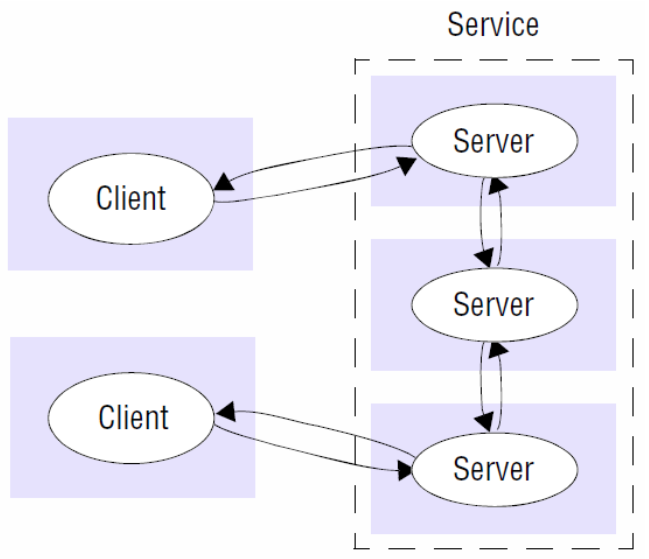
\includegraphics[width=0.45\textwidth]{clientServer.png}
\end{center}

Клиентская часть приложения общается с одним или несколькими сервисами, предоставляющими <<точку входа>> в распределённое приложение --- если это веб-приложение, они же отдают клиенту html-ки и скрипты, которые и составляют клиентскую часть (в том числе по соображениям безопасности --- браузеры сильно ограничивают запросы ко всему, кроме URL, с которых получили страницу). Эти сервисы, в свою очередь, могут вызывать другие сервисы, составляющие приложение, и вместе решать задачу. В больших приложениях таких сервисов могут быть десятки, а то и сотни. В реальной жизни используется некоторая дополнительная инфраструктура --- балансировщики нагрузки, автоматическое масштабирование, системы мониторинга и т.д.

Альтернативными (в каком-то смысле) вариантами размещения являются <<мобильный код>> и <<мобильный агент>>. Мобильный код --- это когда клиент при подключении к серверу получает себе для исполнения код, который делает большую часть содержательной работы на стороне клиента (как правило, в браузере). Так устроены многие современные веб-приложения, например, Google Docs, хотя конкретно в случае Google Docs за мобильным кодом стоит также и большая серверная инфраструктура. Мобильный агент --- это полноценная программа, скачиваемая клиентом и исполняемая на стороне клиента. Используются в основном в peer-to-peer распределённых вычислениях и различных приложениях <<интернета вещей>>, когда данных для обработки много, и доставить код к данным проще, чем собирать данные с оконечных устройств на серверах для обработки.

Также может активно использоваться кеширование, для экономии времени и сетевого трафика при доставке либо данных, либо кода до клиента. Для чего тоже есть широко распространённые готовые решения, например, Redis\footnote{REmote DIctionary Server, \url{https://redis.io/} (дата обращения: 13.10.2021).}.

\section{RPC}

Рассмотрим теперь конкретные технологии организации сетевого взаимодействия компонентов, и начнём с RPC/RMI-инструментов. Все системы удалённого вызова принципиально устроены как на рисунке:

\begin{center}
    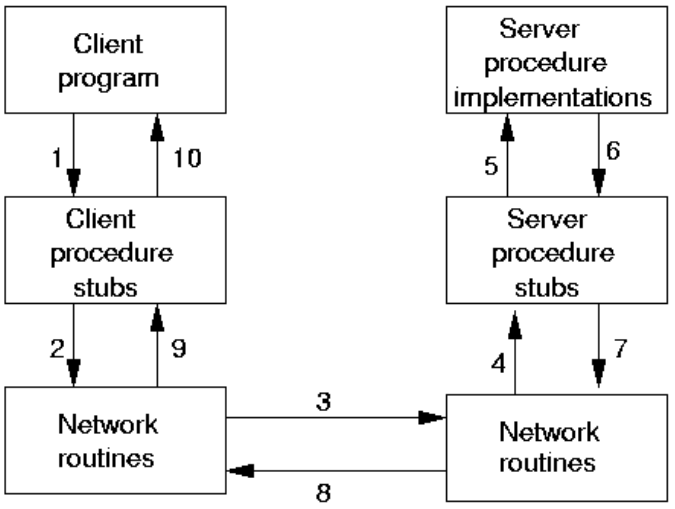
\includegraphics[width=0.45\textwidth]{rpc.png}
\end{center}

При этом программисты пишут только самые верхние блоки --- клиентскую программу и реализации процедур на сервере, которые мы хотим вызывать через RPC. Ещё нужно описать интерфейс сервера --- как правило, в каком-то языконезависимом формате, по которому потом RPC или RMI-система сгенерирует \emph{заглушки} для клиента и для сервера на нужном языке программирования. Клиентские заглушки внешне выглядят как обычный класс, с методами, которые должны быть у соответствующего класса на сервере. Клиентский код может создать заглушку, передать ей каким-то образом адрес и порт сервера (возможно, параметры, нужные для аутентификации/авторизации), и начать вызывать методы как обычно. При этом сгенерированный в заглушке код берёт на себя установление и поддержание сетевого соединения, сериализацию/десериализацию параметров и возвращаемых результатов, передачу данных по сети (используя сетевой стек операционной системы). На сервере всё происходит в обратную сторону --- серверная заглушка, получая сетевой запрос, десериализует параметры, находит и вызывает нужный метод, написанный автором сервера, сериализует ответ, отправляет его по сети обратно.

Светлая цель авторов первых RPC-систем --- чтобы удалённые вызовы были максимально похожи на обычные, так что любой человек, который в состоянии вызвать метод класса, мог бы писать сетевые приложения. При разработке с использованием RPС-систем можно было не думать, на какой машине на самом деле находится тот или иной объект (то, что называется <<location and access transparency>>) --- если на нашей, вызов выполняется как обычно, локально. Если на другой, RPC позаботится обо всех технических деталях и вызов будет выглядеть как обычный.

Однако современная архитектурная мысль сходится к тому, что всё не так просто и различать локальные и удалённые вызовы всё-таки надо. Удалённые вызовы уязвимы к отказам, причём это могут быть отказы самого сервиса (например, он падает при обработке запроса из-за разыменования нулевого указателя) или отказы сети (например, пакет с запросом был потерян перегруженным роутером). И если первый вид отказов критичен для приложения, и надо выдать диагностику клиенту и аккуратно завершить работу, то второй вид отказов надо просто уметь обрабатывать. Есть известная стратегия обработки сетевых отказов --- <<exponential backoff>>, когда мы повторяем запрос, каждый раз увеличивая вдвое время ожидания между попытками, пока запрос не будет успешно исполнен или количество попыток не истечёт. Это позволяет быстро уменьшить частоту запросов, так что если причиной отказа стала перегруженная сеть или перегруженный сервер, общая нагрузка снизится и приложение восстановит работу.

Кроме того, сетевой вызов, в отличие от локального, не мгновенен. Поэтому очень желательно проектировать сетевые вызовы асинхронными, с возможностью отмены операции со стороны клиента. Для локальных вызовов так тоже делают, но только если они могут быть реально длительными, в сетевом же случае каждый запрос может остановить клиент на несколько секунд, если выполняется не асинхронно.

Поэтому многие рекомендуют явно маркировать удалённые вызовы как удалённые, придумав схему именования и используя её консистентно в стиле кодирования. Хотя довольно мало кто так делает на самом деле --- всё-таки удобство RPC-систем и <<прозрачность>> сетевых вызовов весьма привлекательны. Стоит также указывать явно семантику исполнения операции: \emph{at least once} (должна быть исполнена, но спокойно относится к повторам --- как правило, это запросы, не меняющие состояния сервера), \emph{at most once} (операция может быть исполнена не более одного раза, но потеря запроса допустима --- применяется в ситуациях, когда клиент может легко понять, что операция не исполнена, и повторить её), \emph{exactly once} (операция должна быть исполнена обязательно и ровно один раз --- эту семантику труднее всего реализовать в условиях ненадёжной сети, но зачастую необходимо).

RMI (Remote Method Invocation) --- это тот же RPC, но знающий об объектно-ориентированном программировании. Поскольку большинство современных систем пишутся в объектно-ориентированном стиле, многие веб-сервисы реализуются с использованием той или иной RMI-технологии (в большей или меньшей степени RMI). Почему не все --- RPC-системы легковеснее, проще в использовании, быстрее и надёжнее в работе, так что для несложных сервисов предпочтительнее. А поскольку нынче в моде микросервисные архитектуры, где все сервисы должны быть как можно более несложными, RPC-системы популярны. RMI, однако же, более приятны при разработке больших информационных систем: они умеют исключения, иногда умеют распределённые ссылки на объекты (то есть в качестве идентификатора объекта используется не указатель на него в памяти, поскольку память на разных машинах разная и указатели бесполезны, а некий <<глобальный>> идентификатор), ссылки можно передавать как параметры и возвращать как результаты:

\begin{center}
    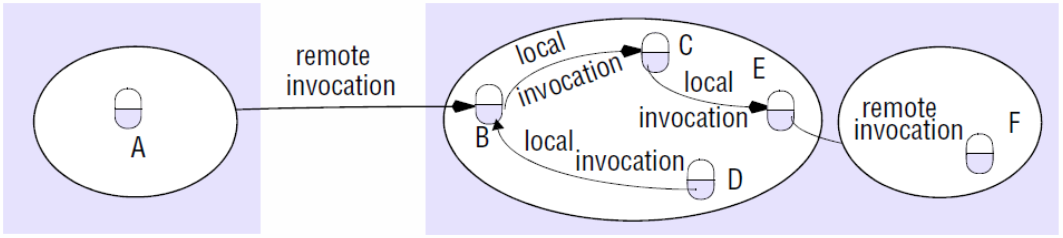
\includegraphics[width=0.8\textwidth]{remoteCalls.png}
\end{center}

Некоторые продвинутые RMI-системы умеют даже распределённую сборку мусора, но автору не приходилось с такими работать.

\subsection{protobuf}

Рассмотрим типичный и активно использующийся в индустрии пример RPC-системы --- Google gRPC. Но поскольку gRPC использует в качестве протокола сериализации протокол от Google, который называется protobuf, сначала кратко рассмотрим его.

Google Protocol Buffers (более известный как protobuf) --- это бинарный формат сериализации произвольных данных. Разработан для внутренних нужд сервисов Google, с целью сэкономить трафик и время передачи. Ближайшие аналоги (XML и JSON) хранят данные в текстовом виде, что хорошо в плане отладки, поскольку они человекочитаемы, но не очень хорошо в плане эффективности передачи или места на диске. protobuf же сериализует данные в хитрый бинарный формат (см. \url{https://developers.google.com/protocol-buffers/docs/encoding}, особого внимания заслуживает способ хранения целых чисел --- Base 128 Varints), что позволяет, по их заявлениям, хранить данные в среднем в 10 раз компактнее формата XML. За это, естественно, надо платить --- protobuf-сообщение не содержит в себе практически никакой информации о своей структуре, передаются только номера полей и значения, при этом чтобы однозначно разобрать сообщение, надо знать типы полей, описанные отдельно.

Это самое отдельное описание --- декларативное описание структуры сообщения в файле .proto, по которому генерируется код для чтения/записи сообщения. Вот пример .proto-файла:

\begin{minted}{protobuf}
syntax = "proto3";

message Person {
    string name = 1;
    int32 id = 2;
    string email = 3;
}
\end{minted}

Версий protobuf бывает две --- proto2 и proto3, с небольшими синтаксическими отличиями, в реальности используются обе (подробности про отличия --- см. в документации). Инструменты поддерживают обе версии протокола, но первой строкой надо указывать версию протокола. Дальше идёт одно или несколько описаний форматов сообщений (в нашем примере --- Person). Сообщения состоят из полей, у каждого поля есть имя, тип и номер. Номера нужны для поддержки изменений в формате записи --- сервер, получив сообщение с незнакомыми полями, может их спокойно проигнорировать. Номера полей есть в любой подобной технологии (например, Apache Thrift описывает формат передачи похожим образом), поскольку протоколы связи имеют свойство эволюционировать, и поддержание обратной совместимости в распределённых приложениях весьма важно.

Ещё protobuf умеет типы-перечисления, массивы/списки (с помощью ключевого слова repeated), вложенные сообщения, импорт сообщений из других файлов, даже что-то вроде вариантных записей (с помощью ключевого слова oneof). В общем, довольно развитый мини-язык программирования для описания данных.

На .proto-файлы во время сборки приложения напускается генератор protoc, который генерирует код под целевой язык программирования. Например, для Java он генерирует класс, представляющий сообщение, и строитель (паттерн <<Строитель>>), который позволяет удобно сообщение сформировать. Поддерживать эти файлы не надо, и даже смотреть на них не надо, они перегенерятся после каждой сборки. В клиентском коде пользоваться ими можно, например, вот так:

\begin{minted}{java}
Person john = Person.newBuilder()
    .setId(1234)
    .setName("John Doe")
    .setEmail("jdoe@example.com")
    .build();
output = new FileOutputStream(args[0]);
john.writeTo(output);
\end{minted}

Builder-у передаются значения полей, дальше методом build() он делает собственно сообщение, у которого есть метод writeTo, принимающий поток, куда надо записать байтовый массив с сериализованным сообщением. Обычно это сетевой поток, но никто не мешает писать protobuf-сообщения на диск (это вполне валидный и весьма компактный формат сохранения), или вообще куда угодно.

protoc обычно подключается как дополнительный компилятор средствами системы сборки. Например, для gradle и maven есть плагины, укачивающие при сборке protoc как maven-пакет, запускающие его на все .proto-файлы, и подключающие результат генерации как обычные Java- или Kotlin-файлы в проект перед запуском обычного компилятора. То есть настройка процесса сборки --- это просто скопировать несколько строк в свой файл с конфигурацией сборки, ничего качать и устанавливать не нужно. Более-менее аналогично оно работает и для других языков (в C++, правда, так и нет пока стандартного пакетного менеджера, там protoc подключить посложнее). Поддерживаются языки Java, Python, Kotlin, Objective-C, C++, Go, Ruby, C\#, Dart.

\subsection{gRPC}

protobuf --- это лишь формат сериализации, так что для написания распределённых систем используется обычно вместе с gRPC, который работает поверх protobuf и даже реализован как расширение к компилятору protoc. gRPC уже позволяет описать сервис в терминах поддерживаемых методов, форматы параметров и возвращаемого результата каждого метода в виде protobuf message. Так же, как в protobuf, описание сервиса языконезависимое, на него потом запускается генератор, порождающий клиентскую или сервисную заглушку на целевом языке. Так же, как и protobuf, gRPC поддерживает кодогенерацию в Java, Python, Kotlin, Objective-C, C++, Go, Ruby, C\#, Dart. gRPC нынче весьма популярен, во-первых, благодаря тому, что Google его сам активно использует в своей инфраструктуре, во-вторых потому, что это простой и легковесный способ писать распределённые приложения, хотя это именно RPC-система, так что её возможности весьма ограничены. Например, gRPC не умеет наследование message, не умеет даже методы, не возвращающие значение (они симулируются методами, возвращающими библиотечное сообщение Message.Empty).

Вот пример описания несложного gRPC-сервиса\footnote{Следуя туториалу \url{https://grpc.io/docs/languages/java/basics/} (дата обращения: 08.11.2021).}:

\begin{minted}{protobuf}
syntax = "proto3";

option java_multiple_files = true;
option java_package = "io.grpc.examples.routeguide";
option java_outer_classname = "RouteGuideProto";

service RouteGuide {
    rpc GetFeature(Point) returns (Feature) {}
    rpc ListFeatures(Rectangle) returns (stream Feature) {}
    rpc RecordRoute(stream Point) returns (RouteSummary) {}
    rpc RouteChat(stream RouteNote) returns (stream RouteNote) {}
}

message Point {
    int32 latitude = 1;
    int32 longitude = 2;
}

message Rectangle {
    Point lo = 1;
    Point hi = 2;
}

message Feature {
    string name = 1;
    Point location = 2;
}

message FeatureDatabase {
    repeated Feature feature = 1;
}

message RouteNote {
    Point location = 1;
    string message = 2;
}

message RouteSummary {
    int32 point_count = 1;
    int32 feature_count = 2;
    int32 distance = 3;
    int32 elapsed_time = 4;
}
\end{minted}

Тут определяется сервис для туристического приложения, который умеет сообщать о достопримечательностях по данным координатам или в данном прямоугольнике, записывать маршрут (состоящий из маршрутных точек) и аннотировать маршрут, сохраняя на сервер и принимая с сервера заметки относительно интересных точек на маршруте. 

Сначала указывается версия синтаксиса .proto-файла, затем опции для кодогенератора (мы хотим .java-файлы, по одному на каждый класс, enum и т.п., в пакете io.grpc.examples.routeguide, при этом чтобы <<фасадом>> для всего этого был класс RouteGuideProto).

Дальше описание собственно сервиса. Он интересен тем, что показывает все возможные режимы передачи данных --- gRPC поддерживает как протоколы вида <<запрос-ответ>>, так и асинхронные потоки сообщений. GetFeature --- классический метод в режиме <<запрос-ответ>>, мы посылаем на сервис точку и получаем достопримечательность, которая в этой точке находится. ListFeatures работает в потоковом режиме, мы отправляем прямоугольник и получаем стрим, из которого можем вычитывать (возможно асинхронно) сообщения с достопримечательностями. Между клиентом и сервером открывается канал, куда сервер может писать новые сообщения, и клиент по мере их появления в канале может их оттуда вычитывать. Когда сервер хочет сказать, что больше сообщений не будет, он должен в явном виде закрыть канал (чуть позже это будет видно в примере реализации сервиса).

RecordRoute работает <<в другую сторону>> --- клиент открывает канал, куда время от времени может писать сообщения, а сервер их асинхронно вычитывает. Когда клиент закончил передачу (например, мы доехали до конечной точки маршрута), он должен явно сообщить об этом серверу, и канал будет закрыт. После этого сервер формирует и отправляет клиенту ответ (одно сообщение на сей раз). RouteChat работает в обе стороны --- между клиентом и сервером открывается канал, куда и клиент и сервер могут писать сообщения независимо друг от друга, вычитывая их асинхронно. Тут уже любая сторона может инициировать закрытие соединения.

Дальше идут описания форматов сообщений, используемых сервисом (и, в случае FeatureDatabase, заодно и используемых сервером для сохранения данных на диск, судя по всему).

Когда мы сгенерируем код серверной части, запустив protoc (в Java за нас это сделает соответствующий плагин к Maven или Gradle), получим серверную заглушку RouteGuideGrpc.RouteGuideImplBase, в которой реализована вся сетевая часть и объявлены виртуальные методы, по одному на каждый метод сервиса из .proto-файла, которые нам надо реализовать. Вот так может выглядеть реализация GetFeature:

\begin{minted}{java}
private static class RouteGuideService extends RouteGuideGrpc.RouteGuideImplBase {
    ...
    @Override
    public void getFeature(Point request, StreamObserver<Feature> responseObserver) {
        responseObserver.onNext(checkFeature(request));
        responseObserver.onCompleted();
    }
    ...
}
\end{minted}

Этот метод работает в режиме <<запрос-ответ>>, поэтому принимает прямо объект типа Point (его десериализует из protobuf-запроса как раз RouteGuideImplBase при получении запроса от клиента по сети). А вот чтобы вернуть ответ, мы должны воспользоваться классом \mintinline{java}{StreamObserver<Feature>}. У StreamObserver всего три метода --- onNext(), onCompleted() и onError(), и по сути это реализация паттерна <<Наблюдатель>>. StreamObserver нотифицируют о наступлении события <<появились новые данные>>, он эти данные сериализует и отправляет по сети на клиент. В данном случае мы должны отправить всего один ответ, поэтому в onNext мы передаём нужные данные (которые для нас готовит не показанный тут доменный метод checkFeature, который просто как-то находит достопримечательности в базе, не важно как). Дальше вызовом onCompleted мы сообщаем об окончании передачи.

Вот так может выглядеть реализация ListFeatures:

\begin{minted}{java}
private static class RouteGuideService extends RouteGuideGrpc.RouteGuideImplBase {
    ...
    @Override
    public void listFeatures(Rectangle request, StreamObserver<Feature> responseObserver) {
        ...
        for (Feature feature : features) {
            int lat = feature.getLocation().getLatitude();
            int lon = feature.getLocation().getLongitude();
            if (lon >= left && lon <= right && lat >= bottom && lat <= top) {
                responseObserver.onNext(feature);
            }
        }
        responseObserver.onCompleted();
    }
}
\end{minted}

Тут передаваемых сообщений уже много, поэтому onNext у responseObserver вызывается в цикле. Но по окончании цикла мы должны вызвать onCompleted, чтобы сообщить клиенту, что передача закончена. Обратите внимание, что никто не заставляет передавать все сообщения сразу, между вызовами onNext может пройти значительное время, клиент будет получать сообщения по мере их готовности.

Вот так может выглядеть реализация RouteChat:

\begin{minted}{java}
@Override
public StreamObserver<RouteNote> routeChat(
        final StreamObserver<RouteNote> responseObserver) {
    return new StreamObserver<RouteNote>() {
        @Override
        public void onNext(RouteNote note) {
            List<RouteNote> notes = getOrCreateNotes(note.getLocation());
            for (RouteNote prevNote : notes.toArray(new RouteNote[0])) {
                responseObserver.onNext(prevNote);
            }
            notes.add(note);
        }

        @Override
        public void onError(Throwable t) {
            logger.log(Level.WARNING, "routeChat cancelled");
        }

        @Override
        public void onCompleted() {
            responseObserver.onCompleted();
        }
    };
}
\end{minted}

Здесь, поскольку канал общения у нас двусторонний, приём и отправка сообщений должны быть симметричны, и поэтому мы и принимаем, и возвращаем StreamObserver. responseObserver, который мы принимаем, как и раньше используется, чтобы писать туда наши данные, которые мы хотим отправить клиенту. Возвращаем мы StreamObserver, который сам gRPC будет дёргать, когда клиент пришлёт нам очередное сообщение. Его метод onNext работает так же, как getFeature и listFeatures --- принимает одно сообщение, что-то с ним делает, и если в результате появляется что-то, что надо передать на клиент, пишет это в responseObserver. В отличие от методов, рассмотренных выше, onCompleted тут не вызывается, поскольку нам могут прислать ещё сообщение и мы должны на него отреагировать. Вот когда клиент сообщит о конце передачи, вызовется наш метод onCompleted, и мы корректно закончим передачу. onError вызовется при возникновении какой-либо ошибки (например, клиент отключился, не сказав <<onCompleted>>).

Обратите внимание, что в этом примере сервер реагирует своим методом onNext на запрос клиента, так что не может <<спонтанно>> послать сообщение. В реальной жизни, однако, ничто не мешает отдать responseObserver в отдельный поток, и генерить события когда и как ему заблагорассудится. Единственное что надо понять, создаёт ли gRPC-сервер уже отдельный поток для слушания клиента или запускается в основном потоке приложения, в клиентах для разных языков это делается по-разному.

Метод RecordRoute мы рассматривать не будем, потому что он устроен аналогично RouteChat: должен вернуть StreamObserver, который бы в onNext ничего не посылал, а в onCompleted делал бы responseObserver.onNext перед responseObserver.onCompleted.

На клиенте генерируются синхронная и асинхронная заглушки, и можно выбрать, какую использовать (конечно асинхронную, синхронные сетевые запросы противоречат идеологии распределённых приложений). Там даже наследоваться ни от чего не надо, а просто дёргать методы этих заглушек так, будто весь RouteService находится в нашем процессе:

\begin{minted}{java}
public class RouteGuideClient {
    private final RouteGuideBlockingStub blockingStub;
    private final RouteGuideStub asyncStub;

    public RouteGuideClient(Channel channel) {
        blockingStub = RouteGuideGrpc.newBlockingStub(channel);
        asyncStub = RouteGuideGrpc.newStub(channel);
    }

    public void getFeature(int lat, int lon) {
        Point request = Point.newBuilder().setLatitude(lat).setLongitude(lon).build();
        
        Feature feature;
        try {
            feature = blockingStub.getFeature(request);
        } catch (StatusRuntimeException e) {
            ...
        }
        if (RouteGuideUtil.exists(feature)) {
            info("Found feature called \"{0}\" at {1}, {2}",
                feature.getName(),
                RouteGuideUtil.getLatitude(feature.getLocation()),
                RouteGuideUtil.getLongitude(feature.getLocation()));
        } else {
            info("Found no feature at {0}, {1}",
                RouteGuideUtil.getLatitude(feature.getLocation()),
                RouteGuideUtil.getLongitude(feature.getLocation()));
        }
    }

    public static void main(String[] args) throws InterruptedException {
        String target = "localhost:8980";
        List<Feature> features = 
            RouteGuideUtil.parseFeatures(RouteGuideUtil.getDefaultFeaturesFile());
        ManagedChannel channel = 
            ManagedChannelBuilder.forTarget(target).usePlaintext().build();
        try {
            var client = new RouteGuideClient(channel);
            client.getFeature(409146138, -746188906);
        } finally {
            channel.shutdownNow().awaitTermination(5, TimeUnit.SECONDS);
        }
    }
    ...
}
\end{minted}

За установление соединения отвечает библиотечный класс ManagedChannelBuilder (часть клиентской библиотеки gRPC для Java), которому надо сказать, куда подключаться (тут это target), что с шифрованием (тут usePlaintext()) и т.п. (тут ничего больше). Дальше мы создаём объект RouteGuideClient, передав ему channel (а то main статический, нам надо сначала <<создать себя>>, чтобы пользоваться нестатическими методами), и вызываем метод getFeature. Конструктор создаст сгенерённые blockingStub и asyncStub, первый из них мы используем в getFeature, передав ему в качестве параметра protobuf-сообщение, полученное с помощью protobuf-builder-а, который мы обсуждали в предыдущем подразделе. Поскольку заглушка синхронная, она тут же отправляет по сети запрос и не возвращает управление, пока не придёт ответ.

Метод RouteChat устроен даже на клиенте более интересно, но рассматривать тут мы его не будем --- у нас будет домашняя работа, предполагающая использование двунаправленного асинхронного канала, так что надо оставить на дом что-то, с чем можно поразбираться самостоятельно. Пример кода и некоторые объяснения есть в туториале, так что думаю, что при желании несложно разобраться.

\section{Веб-сервисы}

Вообще, рассматривать веб-сервисы после RPC-систем и в частности gRPC не очень корректно, потому что RPC --- это всего лишь способ реализации веб-сервисов, тем не менее, обычно предполагается, что веб-сервисы --- более высокоуровневая концепция. Вообще, веб-сервис --- это отдельная система, предоставляющая сетевой интерфейс по какому-либо стандартному протоколу, в стиле RPC или RMI. Веб-сервисы языконезависимы и зачастую даже ожидается, что они независимы от конкретной технологии, хотя в современном мире это не ставится во главу угла (так что gRPC можно назвать механизмом реализации веб-сервисов только с некоторой натяжкой). 

Светлой целью при создании веб-сервисов было иметь стандартный протокол общения, по которому приложения, написанные под самые разные платформы на самых разных технологических стеках, могли взаимодействовать друг с другом. То есть, хотелось получить что-то вроде компонентной модели разработки ПО, только каждый компонент хостится и поддерживается своим производителем и доступен по сети, и чтобы им воспользоваться, надо не покупать целый компонент и мучительно интегрировать его со своим приложением, а купить подписку и платить только за использование. При этом даже предполагалось, что компоненты можно будет легко найти, и затраты на интеграцию (в силу стандартизации протоколов) будут минимальны. В 90-е годы (как раз во время фактического появления настоящей глобальной сети) принимались активные усилия для движения в этом направлении, появлялись стандарты и технологии, и казалось, что вот ещё чуть-чуть --- и программы будут собираться из веб-сервисов как автомобили из запчастей, но... Как и в случае с обычными компонентами (которые были хайпом конца 80-х годов 20-го века), что-то пошло не так, и публичных широкоиспользуемых веб-сервисов общего назначения не так и много. Все пишут свои веб-сервисы (что естественно, поскольку задаи у всех всё-таки специфичные) и деплоят их в своей инфраструктуре (что естественно, вы не хотите оказаться у разбитого корыта, если у кого-то из нужных вам веб-сервисов вырубят интернет). Тем не менее, подавляющее большинство распределённых приложений сейчас --- это набор веб-сервисов, причём и <<своих>>, и сторонних, используемых вместе, зачастую набор довольно большой (даже студенческие работы из более десятка отдельных веб-сервисов у нас бывают, в реальной жизни сервисов могут быть сотни).

С технической точки зрения веб-сервисы обычно используют простые протоколы <<запрос-ответ>> поверх HTTP, где передаются сериализованные во что-то человекочитаемое запросы на вызов методов и параметры для них. Предполагается, что все запросы всегда выполняются асинхронно, и каждый веб-сервис должен корректно обрабатывать как временные отказы, так и ошибки сервисов, с которыми он общается (то есть <<каждый сам за себя>>, независимые отказы). Иногда (в реальной жизни достаточно часто) между сервисами вставляются очереди сообщений, так что сервис посылает запрос не напрямую, а кидает сообщение в очередь и оно доставляется, когда вызываемый сервис готов его обработать. Так же точно реализуются событийные архитектуры --- сервис генерирует события, отправляя их в очередь (или, более в общем, на шину событий --- это не обязательно очередь, может быть общая база данных), кто-то слушает события и реагирует на них, отправляя обратно на шину ответы (если надо).

Формат сообщений стандартизован. Нынче обычно используют либо XML, либо JSON. XML популярен в более старых системах (которых сейчас на самом деле большинство): протоколы SOAP и XML-RPC базируются на XML. JSON более легковесный и не менее человекочитаемый, поэтому современные сервисы используют в основном его (например, архитектура REST предполагает JSON в качестве формата сериализации и все публичные REST-сервисы, типа того же ВКонтакте или сервисов Google, используют JSON).

\subsection{SOAP-ориентированные сервисы}

В качестве примера рассмотрим сервисы, работающие по протоколу SOAP. SOAP (ранее известный как Simple Object Access Protocol) --- это результат эволюции XML-RPC, появился аж в 1998 году и предназначался для реализации RPC на базе XML-сообщений. На самом деле с SOAP связан целый стек технологий:

\begin{center}
    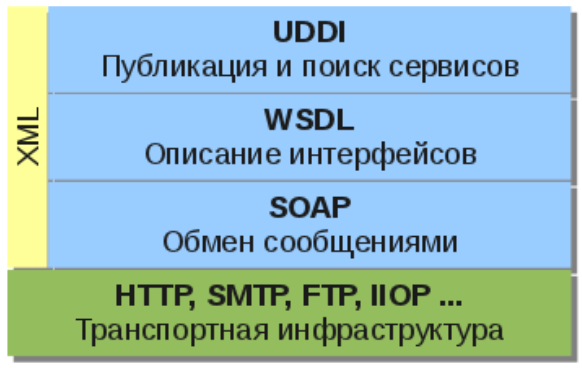
\includegraphics[width=0.35\textwidth]{soap.png}
\end{center}

Сам SOAP отвечает за передачу XML-сообщений поверх транспортного уровня (обычно HTTP/HTTPS, но можно хоть по почте (SMTP) или файлами (FTP)). С ним обычно используется протокол WSDL, Web Services Description Language --- формат описания возможностей сервиса, тоже в формате XML. WSDL-описание вывешивается рядом с самим сервисом, и если вам надо реализовать для сервиса клиент, вы скачиваете WSDL-файл, парсите его, и там написано, какие методы у сервиса есть, как их вызывать, какие параметры они принимают и что возвращают, какие исключения бросаются. В общем, по смыслу похоже на .proto-файлы gRPC, но WSDL --- это стандарт, поддерживаемый W3C, а не корпоративная разработка. И он более многословен и сложнее в использовании без должной инструментальной поддержки.

Кроме того, есть ещё протокол UDDI (Universal Discovery, Description and Integration) --- это шутка, отвечающая за реестр веб-сервисов (по задумке --- глобальный), где можно найти нужный сервис по ключевым словам, узнать про него всякую разную информацию и узнать, где получить WSDL-ку. UDDI издох где-то в начале 2010-х вместе со светлой идеей сборки приложений из третьесторонних веб-сервисов, однако идея интересная.

SOAP и WSDL, однако, живы и здравствуют до сих пор. SOAP до сих пор один из самых популярных протоколов для внутрикорпоративных информационных систем, где объёмы передаваемых данных не так важны (всё находится в одной локалке), а вот надёжность, расширяемость и сопровождаемость критичны. Вот пример SOAP-сообщения, в котором мы говорим сервису раздубить нас в 6:30 утра:

\begin{minted}{xml}
<env:Envelope xmlns:env="http://www.w3.org/2003/05/soap-envelope">
    <env:Header>
        <n:alertcontrol xmlns:n="http://example.org/alertcontrol">
            <n:priority>1</n:priority>
            <n:expires>2001-06-22T14:00:00-05:00</n:expires>
        </n:alertcontrol>
    </env:Header>
    <env:Body>
        <m:alert xmlns:m="http://example.org/alert">
            <m:msg>Get up at 6:30 AM</m:msg>
        </m:alert>
    </env:Body>
</env:Envelope>
\end{minted}

Содержательная часть тут --- только тэг m:msg, но всё сообщение должно быть обёрнуто в SOAP-конверт (тэг Envelope), у которого есть Header и Body, в Header всякая метаинформация, типа приоритета и времени жизни пакета, плюс еще пространства имён XML, которые описывают используемые тэги. protobuf-сообщения, конечно, гораздо компактнее, а JSON сообщения и компактнее, и более человекочитаемы. Зато SOAP позволяет делать весьма продвинутую валидацию ещё до того, как вызовется обработчик сообщения на сервере, считается, что это повышает общую надёжность системы (например, некорректно составленные сообщения не будут соответствовать XML-схеме, которую можно описать в .xsd-документе, и будут отброшены ещё на этапе парсинга).

Руками такие штуки писать тяжело, поэтому для отладки SOAP-сервисов используются инструменты, например, SoapUi\footnote{ДОмашняя страница SoapUi, \url{https://www.soapui.org/} (дата обращения: 08.11.2021).}. С ними всё не так страшно, они даже умеют получить WSDL-ку и сгенерить большую часть запроса за вас. И заодно SoapUi может использоваться для интеграционного тестирования SOAP-ориентированных API, так что для тестировщиков и QA Automation это вообще незаменимый инструмент.

Вот, кстати, как выглядит типичная (очень маленькая) WSDL-ка:

\begin{minted}{xml}
<message name="getTermRequest">
    <part name="term" type="xs:string"/>
</message>

<message name="getTermResponse">
    <part name="value" type="xs:string"/>
</message>

<portType name="glossaryTerms">
    <operation name="getTerm">
        <input message="getTermRequest"/>
        <output message="getTermResponse"/>
    </operation>
</portType>
\end{minted}

Тут описывается один метод, getTerm (видимо, некоего глоссария, который умеет принимать какой-то термин и отдавать его описание). У getTerm есть один аргумент и одно возвращаемое значение. Форматы запроса и ответа описаны выше, с помощью тэгов message. Сравните с gRPC опять-таки --- более многословно, но общая идея такая же.

Итак, достоинства и недостатки SOAP-сервисов.

\begin{itemize}
    \item[+] Автоматическая генерация заглушек на клиенте по WSDL-описанию.
    \item[+] Автоматическая генерация WSDL-описаний по описанию сервиса на обычном языке программирования (если ваш инструмент так умеет, см. ниже про WCF).
    \item[+] Автоматическая валидация сообщений: валидация на уровне парсера XML (если вдруг тэг не закрыт, то всё), валидация на уровне XSD\footnote{XML Schema Document} (что все тэги имеют все нужные атрибуты правильных типов и только разрешённые дочерние тэги), валидация самим сервисом (уже семантики запроса) --- вручную надо делать только последнее.
    \item[+] SOAP использует HTTP как транспорт, поэтому вы можете хоть прямо в браузере просматривать и WSDL, и SOAP-пакеты. Даже посылать запросы, если сможете сделать GET-запрос с Body. Причём, всё человекочитаемо, в отличие от gRPC.
    \item[+] Главное, SOAP стандартный, его все умеют.
    \item[-] Огромный размер сообщений --- оверхед  на всякие пространства имён, обязательные тэги и т.д. и т.п.
    \item[-] Если инструменты всё-таки не поддерживают автоматическую генерацию, писать WSDL руками тяжело.
    \item[-] SOAP не поддерживает транзакции (но, справедливости ради, распределённые транзакции до сих пор никто особо не поддерживает). И на самом деле, модель <<запрос-ответ>>, поддерживаемая SOAP, даже менее выразительна, чем gRPC с его стримами. Но, в принципе, и транзакции, и другие виды сложного взаимодействия можно сделать и вручную, но это потребует усилий и аккуратного проектирования.
    \item[-] При изменении сервиса тяжело мигрировать клиенты (опять-таки, это общая проблема --- если вы контролируете всю систему, то можете их поправить, но если ваш сервис открытый, то даже через 20 лет придёт кто-то с клиентом версии 1.0 и будет жаловаться, что у него не работает). SOAP тут, опять-таки, проигрывает даже gRPC, где хоть какие-то механизмы поддержки обратной совместимости есть. SOAP-ориентированные сервисы решают проблему просто --- запускают все версии сервисов параллельно на разных эндпойнтах (что, впрочем, и для других видов сервисов вполне употребимая практика, например, Google Drive: \url{https://www.googleapis.com/drive/v3} и \url{https://www.googleapis.com/drive/v2}).
\end{itemize}

\subsection{Windows Communication Foundation}

Довольно типичный пример технологии, реализующей SOAP --- это Windows Communication Foundation, библиотека (точнее, фреймворк) для .NET, которая должна была быть основой всей сетевой коммуникации в .NET-программах, но нынче постепенно вытесняется более простыми штуками типа нового ASP.NET Web APIs. Появилась в .NET 3 (примерно 2006 год), исправно служила человечеству до выхода .NET Core, после чего её некоторое время мучительно переписывали на новую платформу и таки переписали (даже выложили в Open Source: \url{https://github.com/dotnet/wcf}). Но, в общем-то, интересна она прежде всего тем, что она используется в корпоративных системах на базе .NET Framework до сих пор очень активно и на её базе сделаны более молодёжные штуки типа того же ASP.NET.

WCF преназначается для быстрого создания веб-сервисов и клиентов для них. Архитектурно она устроена как конфигурируемый фреймворк, состоящий из трёх крупных компонентов: Address, Binding и Contract (так называемые ABCs of WCF). Каждый из компонентов имеет набор абстрактных классов и стандартные их реализации, но можно реализовать и свои, и в конфигурации подсунуть их библиотеке. Так что SOAP не обязателен, можно сделать хоть транспорт на голубиной почте.

\begin{center}
    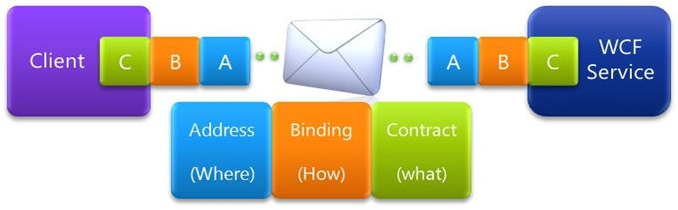
\includegraphics[width=0.6\textwidth]{wcf.png}
    \attribution{\url{http://www.c-sharpcorner.com}}
\end{center}

Address отвечает за понятие эндпойнта сервиса и вообще адресацию. Поскольку на одной машине (и даже на одном порту) может быть запущено сразу много сервисов, различаются они URL-ами (обычно частями после слеша).

Binding отвечает за транспорт --- транспортный протокол, протокол сериализации, безопасность и подобные вещи.

Contract отвечает за исполнение запроса --- либо вызов кода реализации серсива, либо вызов заглушки, которая должна передать запрос по сети. Именно в этом компоненте реализованы атрибуты, размечающие обычный код на C\# так, что по нему потом можно сгенерить WSDL и вызывать по сети\footnote{это пример из официальной документации, так что подробности можно посмотреть там.}: 

\begin{minted}{csharp}
[ServiceContract(Namespace = "http://Microsoft.ServiceModel.Samples")]  
public interface ICalculator  
{
    [OperationContract]
    double Add(double n1, double n2);

    [OperationContract]
    double Subtract(double n1, double n2);

    [OperationContract]
    double Multiply(double n1, double n2);

    [OperationContract]
    double Divide(double n1, double n2);
}
\end{minted}

ServiceContract говорит, что этот интерфейс должен быть доступен как веб-сервис, OperationContract --- что данный метод должен быть методом сервиса. Если бы у методов были аргументы не элементарных типов, потребовались бы ещё атрибуты DataContract --- чтобы пометить контракты данных (типа message в protobuf, опять-таки).

Дальше этот контракт можно реализовать, уже без всяких атрибутов:

\begin{minted}{csharp}
public class CalculatorService : ICalculator  
{
    public double Add(double n1, double n2)
        => n1 + n2;  

    public double Subtract(double n1, double n2)
        => n1 - n2

    public double Multiply(double n1, double n2)  
        => n1 * n2;

    public double Divide(double n1, double n2)  
        => n1 / n2;
}
\end{minted}

А дальше сказать при старте приложения, что такой-то контракт реализуется таким-то классом, хостится на таком-то URL-е и что про него надо вывесить в сеть его WSDL:

\begin{minted}{csharp}
static void Main(string[] args) 
{
    var baseAddress = new Uri("http://localhost:8000/ServiceModelSamples/Service");
    var selfHost = new ServiceHost(typeof(CalculatorService), baseAddress);

    try {
        selfHost.AddServiceEndpoint(typeof(ICalculator), 
            new WSHttpBinding(), "CalculatorService");

        var smb = new ServiceMetadataBehavior();
        smb.HttpGetEnabled = true;
        selfHost.Description.Behaviors.Add(smb);

        selfHost.Open();
        Console.WriteLine("The service is ready. Press <ENTER> to terminate service.");
        Console.ReadLine();

        selfHost.Close();  
    } catch (CommunicationException ce) {
        Console.WriteLine($"An exception occurred: {ce.Message}");
        selfHost.Abort();
    }
}
\end{minted}

\url{http://localhost:8000/ServiceModelSamples/Service} --- это эндпойнт, на котором будет наш сервис. ServiceHost --- это веб-сервер внутри процесса (в отличие от внешнего веб-сервера типа IIS или, если не .NET, Apache), он будет слушать порт 8000 нашей машины и все запросы с URL ServiceModelSamples/Service перенаправлять нашему сервису. Как транспорт используется WSHttpBinding (Web Service over HTTP, то есть SOAP на самом деле --- в реальной жизни не стоит его использовать, только HTTPS). ServiceMetadataBehavior отвечает за генерацию и публикацию WSDL-документа, который мы говорим, что должен быть доступен по HTTP тоже. По умолчанию WSDL-документ кладётся рядом с сервисом (точнее, на \url{http://localhost:8000/ServiceModelSamples/Service/wsdl}). Open() запускает всё это дело, дальше мы блокируемся, давая хосту в отдельном потоке делать своё дело, потом закрываем хост.

Обратите внимание, это практически всё, что надо написать для того, чтобы сделать веб-сервис (а всё остальное --- это boilerplate, который сгенерит среда разработки). То есть создание инфраструктурной части SOAP-сервиса, если знать, что делать, и пользоваться подходящей IDE --- это минут 10 разработки и даже проще чем gRPC на Java.

Со стороны клиента первое, что надо сделать --- это сгенерировать клиентскую заглушку. Для этого сервис должен быть запущен и WSDL-описание доступно для скачивания (на самом деле, это опционально, .wsdl-файл можно хоть по почте прислать). В Visual Studio достаточно нажать <<Add service reference>>, указать URL и выбрать пару опций. Если Visual Studio нет (например, разработка идёт под Linux), есть консольные утилиты из .NET SDK, в частности, svcutil:

\begin{minted}{text}
svcutil.exe /language:cs /out:generatedProxy.cs ^
    /config:app.config http://localhost:8000/ServiceModelSamples/service
\end{minted}

Тут мы говорим, что хотим сгенерировать клиентский прокси в файл generatedProxy.cs на языке C\# (никакой интриги), конфигурацию для него в app.config (это на самом деле XML-файл, про который чуть позже), а сам сервис находится по адресу \url{http://localhost:8000/ServiceModelSamples/service}. Дальше сгенерированную заглушку подключаем к проекту и пишем примерно такой код, чтобы ей воспользоваться: 

\begin{minted}{csharp}
static void Main(string[] args)
{
    var client = new CalculatorClient();

    double value1 = 100.00D;
    double value2 = 15.99D;
    double result = client.Add(value1, value2);
    Console.WriteLine($"Add({value1},{value2}) = {result}");

    client.Close();
}
\end{minted}

И, собственно, всё. Кажется, что какая-то магия --- в gRPC нужно ChannelBuilder, всякие страшные параметры передавать, а тут просто создали заглушку и вперёд. На самом деле, всё дело в app.config, который должен лежать в рабочей папке программы в момент её запуска, там-то всё и написано: 

\begin{minted}{xml}
<?xml version="1.0" encoding="utf-8" ?>  
<configuration>  
    <startup>   
        <supportedRuntime version="v4.0" sku=".NETFramework,Version=v4.5,Profile=Client" />  
    </startup>  
    <system.serviceModel>  
        <bindings>  
            <wsHttpBinding>  
                <binding name="WSHttpBinding_ICalculator" />  
            </wsHttpBinding>  
        </bindings>  
        <client>  
            <endpoint 
                address="http://localhost:8000/ServiceModelSamples/Service/CalculatorService"  
                binding="wsHttpBinding" bindingConfiguration="WSHttpBinding_ICalculator"  
                contract="ServiceReference1.ICalculator" name="WSHttpBinding_ICalculator">  
            </endpoint>  
        </client>  
    </system.serviceModel>  
</configuration>
\end{minted}

Руками такое писать страшновато, но нам его сгенерил svcutil, так что если настройки по умолчанию нас устраивают, то можно на него и не смотреть даже. Из интересного тут тэг endpoint, где указаны address, binding и contract, так что если что-то из этого поменяется, надо будет поправить конфиг, не пересобирая приложение. Обратите внимание на хитрую схему с wsHttpBinding --- параметр binding на самом деле ссылается на отдельной описание байндинга. Дело в том, что на самом деле байндинг может иметь много параметров (те же параметры безопасности, например) и несколько разных конфигураций, поэтому он вынесен в отдельный тэг.

Вот теперь точно всё, это полная клиентская часть.

\section{Очереди сообщений}

Мы пока что рассматривали ситуацию, когда клиент и сервер соединяются напрямую. Часто это может приводить к неприятным ошибкам просто из-за кратковременных сетевых отказов, а часто просто не нужно --- мы хотим всего лишь отправить сообщение в надежде, что оно будет обработано когда-то в будущем (например, послать нотификацию по почте --- сейчас или через полчаса, в случае с электронной почтой обычно разницы нет). В качестве прослойки между клиентом и сервером можно использовать очереди сообщений --- системы, обеспечивающие гарантированную доставку сообщений, даже если отправитель и получатель в разное время находятся в онлайне. Обычно очередь сообщений --- это отдельный сервер (который простой и не самодельный, поэтому, скорее всего, у него будет высокий аптайм), либо локальное хранилище сообщений у каждого отправителя. Отправитель не шлёт сообщение непосредственно серверу, а кладёт его в очередь, и сервер, когда готов, забирает его оттуда (либо очередь сама время от времени пытается его доставить, в зависимости от архитектуры конкретной системы).

Очереди сообщений позволяют нескольким отправителям писать сообщения, и нескольким получателям, соответственно, читать, так что позволяют организовать более интересные способы взаимодействия, чем <<точка-точка>> (хотя в этом качестве тоже активно используются). Например, очередь сообщений может реализовывать модель <<издатель-подписчик>>, когда один источник кидает в неё события, а несколько подписчиков вычитывают (при этом, в зависимости от задачи, одно сообщение может доставляться всем подписчикам, а может и только одному --- так, например, можно балансировать нагрузку в распределённых вычислительных системах). Очередь также может выступать в роли шины событий для событийно-ориентированных архитектур --- все, кто производят события, пишут события в очередь (может, в несколько разных очередей, по одной на каждый тип события), все, кто хочет слушать события, просто забирают их из очереди (опять-таки, удаляя событие из очереди или нет).

Очереди при этом обычно имеют развитые возможности по маршрутизации, фильтрации и преобразованию сообщений, реализованные на стороне собственно очереди. Например, разветвители, которые раскидывают сообщения из одной очереди по нескольким, агрегаторы, которые, наоборот, сливают сообщения из нескольких очередей в одну, преобразователи порядка, которые могут переставлять или сортировать сообщения.

Реализаций очередей сообщений довольно много, достойна упоминания, например, MSMQ (Microsoft Message Queuing), очередь сообщений, поставляемая прямо с Windows. Так что если вы не имели идей, что такое очереди сообщений, у вас наверняка есть или когда-то был компьютер, где очередь сообщений была и даже работала. Кстати, MSMQ поддерживается в WCF как Binding.

\subsection{RabbitMQ}

Одна из самых популярных реализаций очередей сообщений --- RabbitMQ\footnote{Домашняя страница RabbitMQ, \url{https://www.rabbitmq.com/} (дата обращения: 08.11.2021).}, называемая на жаргоне <<кролик>>. Это как раз реализация с отдельным сервером (написанным, внезапно, на Erlang, так что чтобы RabbitMQ заработала, ей нужен Erlang runtime). Клиент при отправке сообщения подключается по сети к серверу (никто не мешает задеплоить его на той же машине, что и клиент, впрочем) и сохраняет сообщение там. Сообщение хранится, возможно, будучи записанным на диск, чтобы пережить даже перезапуск сервера RabbitMQ. Когда получатель готов его обработать, он подключается к серверу, указывает из какой очереди забрать сообщение и удалить ли его после обработки, и забирает сообщение. RabbitMQ никакой кодогенерации не использует, сообщения для неё --- просто массивы байтов (что, кстати, даёт возможность сериализовать сообщения в формат protobuf, например). Клиентские библиотеки доступны практически для любых языков программирования.

RabbitMQ реализует стандартный протокол AMQP (Advanced Message Queuing Protocol), так что теоретически может работать и со сторонними клиентами, и интегрироваться с другими очередями. Но не уверен, что кто-то пробовал. RabbitMQ имеет развитые возможности по маршрутизации сообщений --- на самом деле, сообщение добавляется не в очередь вовсе, а в exchange --- именованный и конфигурируемый маршрутизатор, который по умолчанию тут же пересылает сообщение в очередь с таким же именем и больше ничего не делает (так что пользоваться RabbitMQ можно, даже не зная про существование exchange-ей). Однако ему можно сказать раскидывать сообщения по разным очередям, маршрутизовать сообщения по ключам, отправляемым с сообщением клиентом, фильтровать сообщения и творить прочие хорошие вещи.

Но перейдём к примеру кода. Вот отправитель (на C\#):

\begin{minted}{csharp}
using System;
using RabbitMQ.Client;
using System.Text;

class Send
{
    public static void Main()
    {
        var factory = new ConnectionFactory() { HostName = "localhost" };
        using var connection = factory.CreateConnection();
        using var channel = connection.CreateModel();
        channel.QueueDeclare(queue: "hello", durable: false, exclusive: false,
                autoDelete: false, arguments: null);

        string message = "Hello World!";
        var body = Encoding.UTF8.GetBytes(message);

        channel.BasicPublish(exchange: "", routingKey: "hello",
                basicProperties: null, body: body);
    }
}
\end{minted}

Создаём подключение, сообщая ConnectionFactory имя хоста, на котором запущен сервер. Порт указывать не надо, он по умолчанию 5672. Дальше создаём канал --- канал представляет виртуальное соединение по протоколу AMPQ внутри физического подключения, которое описывается классом Connection. Теоретически один Connection может поддерживать несколько каналов. Дальше мы внутри канала объявляем очередь с именем <<hello>>, говорим (durable: false), что она должна сохранять сообщения только в память, а не на диск (так менее надёжно, но быстрее), что очередь не надо удалять при закрытии соединения (exclusive: false), что очередь не надо удалять, когда читатель от неё отписывается (autoDelete: false), не передаём дополнительных аргументов. Если очередь с таким именем на сервере уже есть, QueueDeclare ничего не делает, однако если параметры очереди не совпадают, RabbitMQ вернёт ошибку. Дальше мы сериализуем наше сообщение и публикуем его в очередь (методом BasicPublish) с ключом <<hello>>, по которому exchange поймёт, что его надо отправить в очередь <<hello>>.

Теперь получатель:

\begin{minted}{csharp}
using RabbitMQ.Client;
using RabbitMQ.Client.Events;
using System;
using System.Text;

class Receive
{
    public static void Main()
    {
        var factory = new ConnectionFactory() { HostName = "localhost" };
        using var connection = factory.CreateConnection();
        using var channel = connection.CreateModel();
        channel.QueueDeclare(queue: "hello", durable: false, exclusive: false, 
            autoDelete: false, arguments: null);

        var consumer = new EventingBasicConsumer(channel);
        consumer.Received += (model, ea) =>
        {
            var body = ea.Body;
            var message = Encoding.UTF8.GetString(body);
            Console.WriteLine(" [x] Received {0}", message);
        };
        channel.BasicConsume(queue: "hello", autoAck: true, consumer: consumer);
    }
}
\end{minted}

Тут тоже, создаём подключение к локалхосту, объявляем очередь (на случай, если получатель будет запущен раньше отправителя, если нет, то QueueDeclare ничего не делает). А дальше мы создаём асинхронного получателя сообщений и запускаем блокирующий метод BasicConsume, указывая ему очередь, которую надо слушать, автоматически подтверждать доставку и удалять сообщение из очереди, ну и consumer, который будет вызываться при появлении в очереди сообщения. Собственно получатель --- это лямбда-функция с двумя аргументами, подписанная на событие Received у consumer. model --- это канал, ea --- собственно полученное сообщение, у него мы берём тело (байтовый массив), десериализуем и печатаем на экран.

Опять-таки, это прямо готовые программы отправителя и получателя, да и сам RabbitMQ с параметрами по умолчанию запустить ничего не стоит (особенно из Docker-контейнера), так что завести это всё в базовом варианте --- дело десяти минут. Впрочем, правильно всё настроить (например, авторизацию по сертификатам --- вы же не хотите, чтобы кто угодно мог подписываться на сообщения или писать сообщения в очередь) может быть уже не так тривиально.

\subsection{Apache Kafka}

Apache Kafka занимает схожую с RabbitMQ экологическую нишу и вполне сравнима с ней по популярности, так что выбор между Kafka и RabbitMQ --- вполне серьёзная задача (хотя часто определяется личными предпочтениями). Kafka использует несколько другой подход к работе с сообщениями, она на самом деле не очередь, а распределённый лог событий. Сообщение в Kafka посылается на сервер в целом так же, как в RabbitMQ, не не вычитывается получателем, а просто записывается и хранится до тех пор, пока политика чистки логов его не удалит (по умолчанию это происходит по таймеру, где-то раз в семь дней, но ничто в принципе не мешает хранить событий хоть вечно). Каждый подписчик по сути просто читает лог, получая сообщения последовательно (как будто бы из стрима), и сам хранит индекс последнего прочитанного сообщения (технически не совсем сам, потому что хочется, чтобы если получатель умрёт, он мог запуститься и продолжить --- так что индекс хранится на сервере, но привязан к получателю). Так что несколько получателей могут вычитывать сообщения независимо, и каждый получатель может отмотать назад индекс и вычитать сообщения снова (чего нельзя в RabbitMQ и что бывает удобно, чтобы повторно проиграть последовательность событий --- например, заново заполнить базу данными).

Делается так для того, чтобы избежать необходимости чрезмерного общения сервера и клиента и достичь практической немутабельности хранимых данных. Что позволяет получить большую выгоду от распределённости --- Kafka может быть запущена на кластере и хранить разные части лога на разных физических машинах, выдавая события читателям параллельно. Да и не только в распределённости дело, такой подход позволяет весьма эффективно хранить данные, поэтому даже один экземпляр Kafka работает быстрее, чем экземпляр RabbitMQ. Кроме того, такой подход хорошо ложится на событийные стили и подход <<Event Sourcing>> --- когда система вообще не хранит состояние, а хранит просто последовательность событий, по которому состояние можно построить. Поэтому Kafka очень популярна там, где состояние не очень важно, событий много, и надо уметь быстро их агрегировать и что-то по ним считать --- например, в разных приложениях <<интернета вещей>>, где оконечные устройства могут сыпать сотнями тысяч событий в минуту. Однако Kafka немного сложнее в настройке и несколько хуже в маршрутизации сообщений, поэтому RabbitMQ популярнее в информационных системах, где событий не очень много, но надёжная доставка адресату (и только ему) критична. Впрочем, не стоит думать, что сценарии типа балансировщика нагрузки на Kafka не реализовать --- в Kafka есть понятие <<группа подписчиков>>, они координируются между собой так, чтобы каждое событие доставлялось только одному участнику группы.

Архитектурно Kafka устроена как набор \emph{брокеров}, обслуживающих запросы издателей и подписчиков, и хранящих каждый свою часть лога:

\begin{center}
    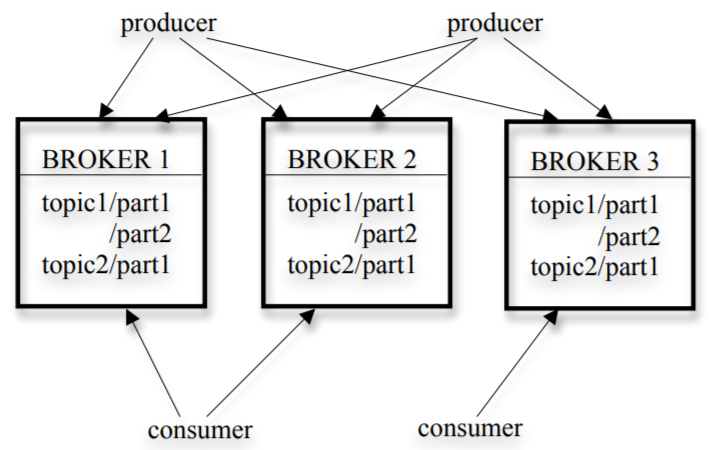
\includegraphics[width=0.6\textwidth]{kafkaArchitecture.png}
    \attribution{J. Kreps et al., Kafka: a Distributed Messaging System for Log Processing, 2011}
\end{center}

Лог разделён на \emph{топики} --- каналы, куда можно писать и откуда можно читать отдельно от других. Топики разделены на \emph{разделы} --- логические куски топиков. Отправитель может послать событие в конкретный раздел, по умолчанию события распределяются равномерно. Кроме того, для события можно указать ключ, тогда раздел, в который оно попадёт, определяется по хешу ключа, так что все сообщения с одним ключом попадут в один раздел. Подписчики из одной группы получают события из разных разделов (см. \url{https://stackoverflow.com/questions/38024514/understanding-kafka-topics-and-partitions}, там хорошее объяснение с картинками). Топики и разделы хранятся на одном или нескольких брокерах, которые балансируют между собой нагрузку и собственно хранят на диске данные (для Kafka принципиально, что на диске --- она даже кеширование в оперативной памяти не использует, надеясь на функциональность кеширования файловой системы --- и товарищи в статье выше говорят, что это реально хорошее решение).

Как обычно, пример кода на C\#, отправитель:

\begin{minted}{csharp}
using Confluent.Kafka;

var config = new ProducerConfig { BootstrapServers = "localhost:9092" };

using var p = new ProducerBuilder<Null, string>(config).Build();
try
{
    var deliveryResult = await p.ProduceAsync(
        "test-topic", new Message<Null, string> { Value = "test" });
}
catch (ProduceException<Null, string> e)
{
    Console.WriteLine($"Delivery failed: {e.Error.Reason}");
}
\end{minted}

Тут мы создали отправителя, который должен связаться с брокером на localhost:9092 (9092 --- стандартный порт Kafka). Дальше мы паттерном <<Строитель>> конфигурируем строитель, который будет отправлять сообщения без ключа (Null) и со значением строкового типа. ProduceAsync асинхронно отправит сообщение на брокер (если не отправится, мы поймаем исключение и поругаемся).

Вот получатель: 

\begin{minted}{csharp}
using Confluent.Kafka;

var conf = new ConsumerConfig {
    GroupId = "test-consumer-group",
    BootstrapServers = "localhost:9092",
    AutoOffsetReset = AutoOffsetReset.Earliest
};

using var consumer = new ConsumerBuilder<Ignore, string>(conf).Build();
consumer.Subscribe("my-topic");

var cts = new CancellationTokenSource();
Console.CancelKeyPress += (_, e) => {
    e.Cancel = true;
    cts.Cancel();
};

try {
    while (true) {
        var consumeResult = consumer.Consume(cts.Token);
        Console.WriteLine($"Consumed message '{consumeResult.Message.Value}'.");
    }
}
catch (OperationCanceledException) {
    consumer.Close();
}
\end{minted}

Получатель более долго настраивается --- ему помимо адреса брокера надо передать идентификатор группы и политику сброса индекса сообщения (которая применяется, при первом запуске, или если на сервере логи подчистились и текущий индекс перестал быть валиден). Тут мы говорим, что хотим начать вычитывать сообщения начиная с первого в топике (если топик сброшен, старые сообщения удалились и мы в любом случае получим то, что ещё не видели). Можно попросить с последнего --- тогда мы при включении не будем вынуждены обрабатывать историю, а сразу начнём получать свежие события.

Дальше опять с помощью паттерна <<Строитель>> создаём получателя, подписываемся на топик <<my-topic>>, создаём токен отмены (это стандартный механизм .NET, позволяющий прерывать асинхронные операции) и запускаем бесконечный цикл потребления сообщений. пока нас не прервут по нажатию на Ctrl-C.

Как видим, в клиентском коде на самом деле даже проще, чем RabbitMQ. Зато если в RabbitMQ достаточно было просто запустить сервер (ну, для базовых сценариев), то в Kafka потребуется их аж два --- сама Kafka и Zookeeper (сервис координации группы брокеров --- вообще, они собираются от него избавиться, вроде, чтобы можно было просто Kafka запускать).

% \section{Redis}

\end{document}